\begin{frame}{Miscellaneous Exercises}
\begin{enumerate}
\conti
\item The length of the
minute hand of a clock is 14 cm. Find the area
swept by the minute hand in 5 minutes.\\
\seti
\end{enumerate}
\begin{itemize}
\item \textbf{Solution} :
\item Given r = 14 
\begin{figure}[!ht]
\resizebox{0.5\linewidth}{!}
{
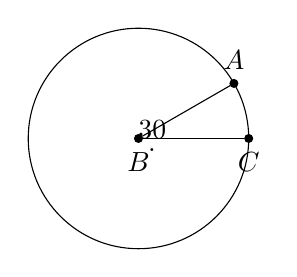
\begin{tikzpicture}
[scale =0.1,>=stealth,point/.style = {draw, circle, fill = black, inner sep = 1pt},]
\node (B) at (0,0)[point,label=below :$B$] {};
\node (C) at (14,0)[point,label=below :$C$] {};
\node (A) at (12.12,6.99)[point,label=above :$A$] {};
\draw (0,0) node [below right] {.} circle (14);
\draw (B)--(A);
\draw (B)--(C);
\tkzMarkAngle[fill=green!40,size=0.1cm,mark=](C,B,A)
\tkzLabelAngle[pos=0.1](C,B,A){\rotatebox{-360}{$30$}}
\end{tikzpicture}


}

\end{figure}


\end{itemize}
\end{frame}
\begin{frame}
\begin{figure}
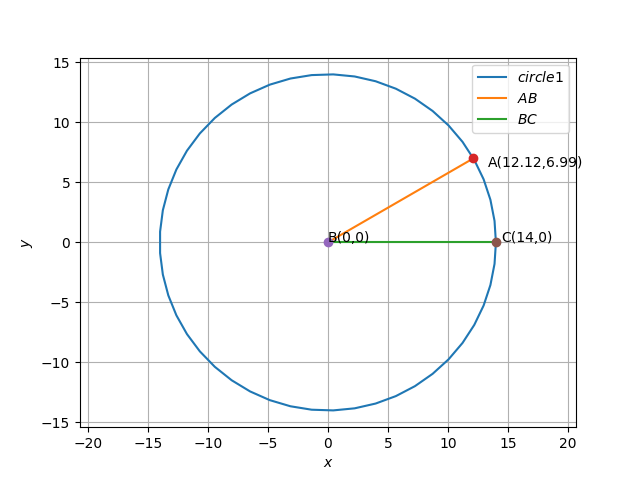
\includegraphics[scale=.6]{./CODES/MISC.png}
\end{figure}
\end{frame}
\begin{frame}

 In 60 minutes minute hand covers  360$\degree$\\
For 5 minutes 6$\degree$ $\times$ 5 = 30$\degree$\\ 
Here $\theta$ = 30 $\degree$ and r = 14cm\\

\begin{align*}
	\text{Area of sector} = \frac{\theta}{360} \times \pi r^2
	=51.31cm^2.
\end{align*}   
\begin{itemize}
\item \url {https://github.com/pratibha444/GEOMETRY/blob/master/figs/clock.tex} 
\item \url{https://github.com/pratibha444/GEOMETRY/blob/master/CODES/newclock.py}
\end{itemize}             
\end{frame}